%!TEX root = ../../../main.tex
%%---------------------------------------------------------------------------
\section{SCRUM \label{sec:scrum}}
%%---------------------------------------------------------------------------

%Description of our way of doing SCRUM...

The Agile methodology suited this project since the iterative development has a good synergy when it comes to customer collaboration and changes in requirements. Two aspects in the system development was influencing the defining of tasks. The first aspect is system requirements were not completely finalized from the beginning. The second aspect is a lot of new unfamiliar technologies and tools made it hard to get a breakdown of the processes required to complete the system.

The project started the 7th of September 2015 with a introduction to the system requirements by the product owners and the system development ended the 7th of December with a 24 hour integration test.

The team gathered after the system requirements were presented in order to create an initial prioritized product backlog. The team utilized Trello \citep{trello} in order to keep track of the tasks in the backlog. Trello is an online project management application and it was used since its design made it similar to post-it notes for management. It also has the advantage of being online and therefore accessible from both home and workplace through smart phones or computers. Figure \ref{fig:trello_cap} shows a screen capture of Trello board for a sprint log.
\begin{figure}[H]
	\centering
	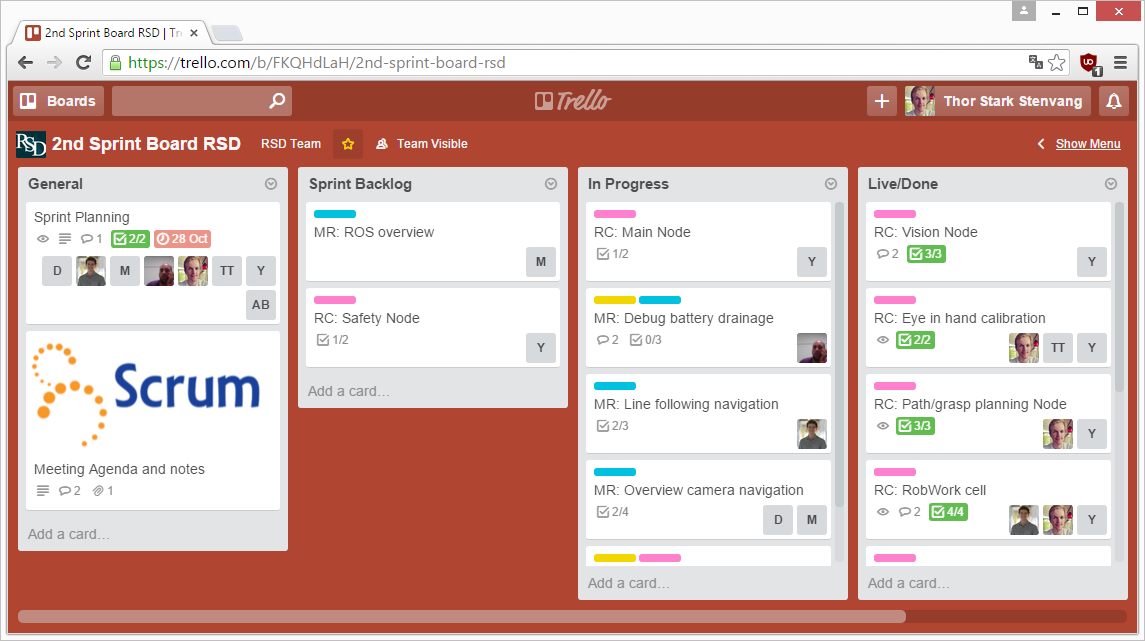
\includegraphics[width=\textwidth]{figs/trello_example.png}
	\caption{Screen capture of a Trello showing the Trello board for the 2nd Sprint. The three rightmost lists are used to keep track of tasks and their state.}
	\label{fig:trello_cap}
\end{figure}

\subsection{Sprints} \label{sec:sprints}
Over the course of the project the work was divided into 4 sprints. Each sprint planning, except the first, was done after the completion of the previous. For each sprint the goal and duration was decided. Prioritized tasks were then added to the \emph{Sprint backlog}. While the \emph{Sprint} was running each member could sign up for tasks and move them from the \emph{"Sprint Backlog"} to \emph{"In Progress"} or \emph{"Live/Done"}, see Figure \ref{fig:trello_cap}. 
Listed below are the different Sprints and their description.

\begin{itemize}
    \item \textbf{1st Sprint.}
    \begin{itemize}
    	\item \textbf{Goal:} Create a working robot demo for the TEK opening and prepare the simple elements for the robot cell.
    	\item \textbf{Duration:} 14th of Sep - 30th of Sep.
    	\item \textbf{Description:} Additional to the system described in the original system requirements, an additional system had to be developed with a release date of 30th of September. The new requirements were the development of a mobile robot able to perform at the TEK opening at University of Southern Denmark. The Sprint was designed with the new requirements and deadline in mind. There were several hardware issues with the robot cell at the beginning of the sprint, and with these two factors the sprint prioritized the development of the mobile platform.
	\end{itemize}
	
    \item \textbf{2nd Sprint.}
    \begin{itemize}
    	\item \textbf{Goal:} Fulfil the requirements for the halfway demonstration.
    	\item \textbf{Duration:} 5th of Oct - 28th of Oct.
    	\item \textbf{Description:} A deadline for a halfway demonstration of the system was set to the 26th of October. This halfway demonstration required several subtask of the system to be complete and the requirements therefore spread the the workforce onto a broader part of the system compared to previous sprint since both mobile robot and robot cell had to be partly finished before demonstration.
	\end{itemize}
	
    \item \textbf{3rd Sprint.}
    \begin{itemize}
    	\item \textbf{Goal:} Get the system ready so all subsystems and components can be integrated together in the next sprint.
    	\item \textbf{Duration:} 28th of Oct - 18th of Nov.
    	\item \textbf{Description:} With most of the work on the robot work cell done in the previous sprint. The workforce was shifted so more people were working on the mobile robot. This allowed the sub-parts to be ready for implementation and integration in the whole system.
	\end{itemize}
	
    \item \textbf{4th Sprint.}
    \begin{itemize}
    	\item \textbf{Goal:} Integrate all subsystems and components and prepare for the 24 hour integration test.
    	\item \textbf{Duration:} 23rd of Nov - 7th of Dec.
    	\item \textbf{Description:} All sub navigation and skills of the mobile robot had to be implemented together so they in conjugation can perform all the defined task for the mobile robot. Additional the whole system had to be tested and finished including the communication with the MES. Additional bug fixes and recovery behaviour were done in order to complete the 24 hour integration test in an environment where other robots are present.
	\end{itemize}
\end{itemize}

In order to keep an overview of the project and keeping it on track a weekly SCRUM meeting was held together with the Consultant and a Product owner.